
\section{Problem Statement}
My team at Statcon Electronics India Ltd has been focusing on enhancing the
efficiency and performance of Switched Mode Power Supplies. Presently, most
SMPS utilize switching of MOSFETs at high frequencies to generate an alternating
high frequency signal which is then passed through a rectifier and filtered using
capacitors.


\section{Overview}

\subsection{Traditional Rectifier}
This is \ref{fig:llc_converter}

\begin{figure}[h]
    \centering
    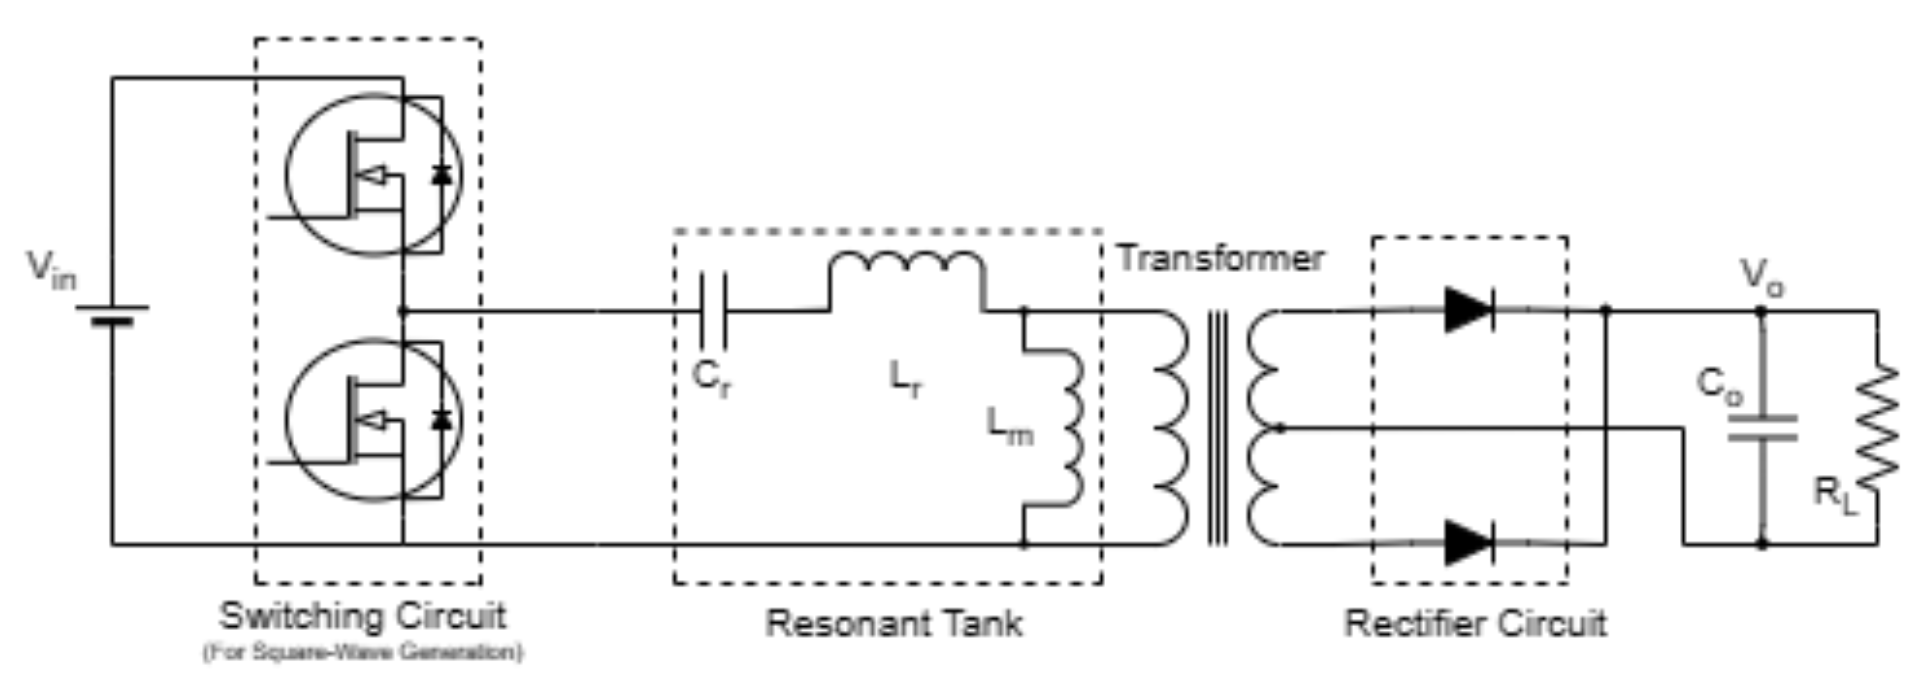
\includegraphics[width=\textwidth]{LLC_converter.png}
    \caption{Diagram of an LLC based resonant converter}
    \label{fig:llc_converter}
\end{figure}

\noindent


\subsection{Vector Control}


\subsection{Space Vector Modulation}


\section{Challenges}
I faced many challenges in developing a Active front-end converter. Firstly,
distinguishing between Sinusoidal Pulse Width Modulation (SPWM) and Space
Vector Pulse Width Modulation (SVPWM) posed confusion due to their perceived
similarity in operational principles. Secondly, reconciling the non-zero
resultant vector in SVPWM with the traditional understanding of three-phase
systems, where the vector sum equals zero, required conceptual clarification to
ensure accurate system design and analysis. Another challenge was comprehending
how rectification and regeneration can occur through the same IGBT bridge, as
it involved bidirectional power flow management. Additionally, not knowing how
to write code in MATLAB was another challenge, but learning it opened up new
possibilities for simulating and analyzing our AFE converter designs.